\section{Equations and Tables}

Equations can be added like so:

\begin{equation}
  \label{eq:sum}
  \sum_{j=1}^{z} j = \frac{z(z+1)}{2}
\end{equation}

Tables, such as \cref{tab:vis-papers} can also be included.

\begin{table}[tb]
  \caption{%
    VIS/VisWeek accepted/presented papers: 1990--2016.%
  }
  \label{tab:vis-papers}
  \scriptsize%
  \centering%
  \begin{tabu}{%
      r%
        *{7}{c}%
        *{2}{r}%
    }
    \toprule
    year         & \rotatebox{90}{Vis/SciVis} & \rotatebox{90}{SciVis conf} & \rotatebox{90}{InfoVis} & \rotatebox{90}{VAST} & \rotatebox{90}{VAST conf} & \rotatebox{90}{TVCG @ VIS} & \rotatebox{90}{CG\&A @ VIS} & \rotatebox{90}{VIS/VisWeek} \rotatebox{90}{incl.\ TVCG/CG\&A} & \rotatebox{90}{VIS/VisWeek} \rotatebox{90}{w/o TVCG/CG\&A} \\
    \midrule
    2016         & 30                         &                             & 37                      & 33                   & 15                        & 23                         & 10                          & 148                                                           & 115                                                        \\
    2015         & 33                         & 9                           & 38                      & 33                   & 14                        & 17                         & 15                          & 159                                                           & 127                                                        \\
    2014         & 34                         &                             & 45                      & 33                   & 21                        & 20                         &                             & 153                                                           & 133                                                        \\
    2013         & 31                         &                             & 38                      & 32                   &                           & 20                         &                             & 121                                                           & 101                                                        \\
    2012         & 42                         &                             & 44                      & 30                   &                           & 23                         &                             & 139                                                           & 116                                                        \\
    2011         & 49                         &                             & 44                      & 26                   &                           & 20                         &                             & 139                                                           & 119                                                        \\
    2010         & 48                         &                             & 35                      & 26                   &                           &                            &                             & 109                                                           & 109                                                        \\
    2009         & 54                         &                             & 37                      & 26                   &                           &                            &                             & 117                                                           & 117                                                        \\
    2008         & 50                         &                             & 28                      & 21                   &                           &                            &                             & 99                                                            & 99                                                         \\
    2007         & 56                         &                             & 27                      & 24                   &                           &                            &                             & 107                                                           & 107                                                        \\
    2006         & 63                         &                             & 24                      & 26                   &                           &                            &                             & 113                                                           & 113                                                        \\
    2005         & 88                         &                             & 31                      &                      &                           &                            &                             & 119                                                           & 119                                                        \\
    2004         & 70                         &                             & 27                      &                      &                           &                            &                             & 97                                                            & 97                                                         \\
    2003         & 74                         &                             & 29                      &                      &                           &                            &                             & 103                                                           & 103                                                        \\
    2002         & 78                         &                             & 23                      &                      &                           &                            &                             & 101                                                           & 101                                                        \\
    2001         & 74                         &                             & 22                      &                      &                           &                            &                             & 96                                                            & 96                                                         \\
    2000         & 73                         &                             & 20                      &                      &                           &                            &                             & 93                                                            & 93                                                         \\
    1999         & 69                         &                             & 19                      &                      &                           &                            &                             & 88                                                            & 88                                                         \\
    1998         & 72                         &                             & 18                      &                      &                           &                            &                             & 90                                                            & 90                                                         \\
    1997         & 72                         &                             & 16                      &                      &                           &                            &                             & 88                                                            & 88                                                         \\
    1996         & 65                         &                             & 12                      &                      &                           &                            &                             & 77                                                            & 77                                                         \\
    1995         & 56                         &                             & 18                      &                      &                           &                            &                             & 74                                                            & 74                                                         \\
    1994         & 53                         &                             &                         &                      &                           &                            &                             & 53                                                            & 53                                                         \\
    1993         & 55                         &                             &                         &                      &                           &                            &                             & 55                                                            & 55                                                         \\
    1992         & 53                         &                             &                         &                      &                           &                            &                             & 53                                                            & 53                                                         \\
    1991         & 50                         &                             &                         &                      &                           &                            &                             & 50                                                            & 50                                                         \\
    1990         & 53                         &                             &                         &                      &                           &                            &                             & 53                                                            & 53                                                         \\
    \midrule
    \textbf{sum} & \textbf{1545}              & \textbf{9}                  & \textbf{632}            & \textbf{310}         & \textbf{50}               & \textbf{123}               & \textbf{25}                 & \textbf{2694}                                                 & \textbf{2546}                                              \\
    \bottomrule
  \end{tabu}%
\end{table}


\begin{figure}[tb]% specify a combination of t, b, p, or h for top, bottom, on its own page, or here
  \centering % avoid the use of \begin{center}...\end{center} and use \centering instead (more compact)
  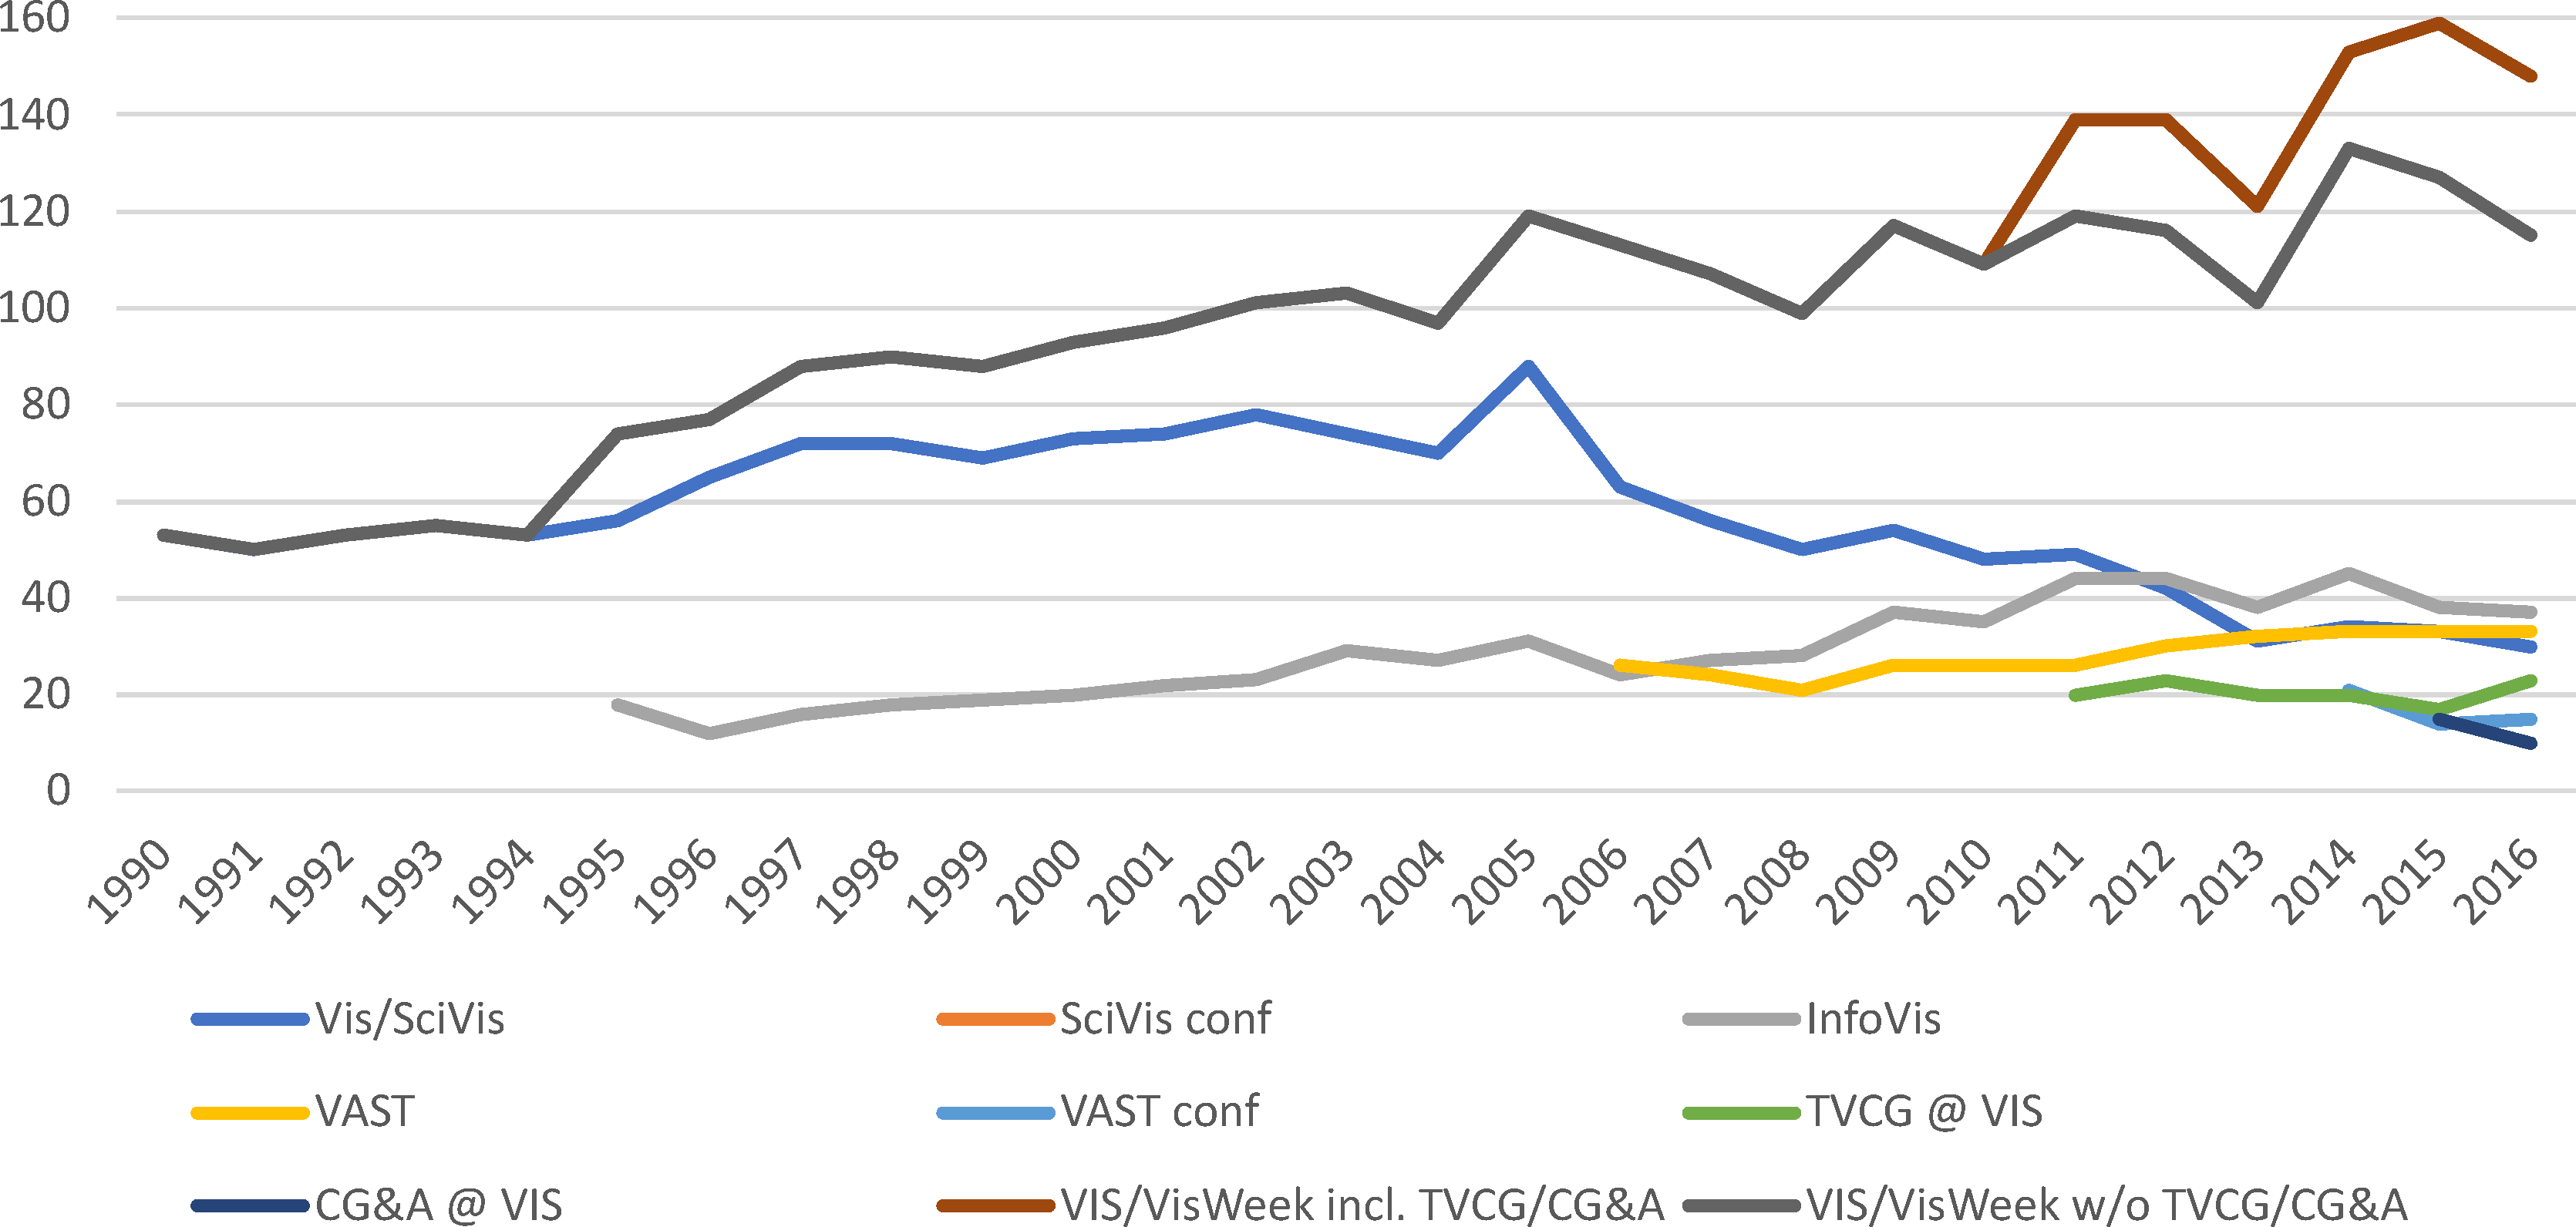
\includegraphics[width=\columnwidth, alt={A line graph showing paper counts between 0 and 160 from 1990 to 2016 for 9 venues.}]{./assets/imgs/2-paper-count-2016/paper-count-2016.pdf}
  \caption{%
  	A visualization of the 1990--2016 data from \cref{tab:vis-papers}, recreated based on Fig.\ 1 from \cite{Isenberg2017Vispubdata.orgMetadataCollection}.%
  }
  \label{fig:vis_papers}
\end{figure}
